\documentclass{article}
\include{preamble}
\title{Project GRASP -- geometry 1}
\author{Adam Kurkiewicz\\
  \small{Univeristy of Glasgow}\\
  \small{adam@kurkiewicz.pl}}
\usepackage[utf8]{inputenc}
\usepackage{graphicx}
%\graphicspath{ {images/} }
 
 
 
\begin{document}
  \maketitle
  \section{Administrative Stuff}
  
  \subsection{Google Classroom}
  Per popular request I've set up a google classroom: https://tinyurl.com/y9nojnfm
  
  The classroom code is: s8xlovo. There isn't much there yet, but from now on I'll be putting all the materials there as opposed to the mailing list.
  
  \subsection{Olympiad problems}
  \begin{enumerate}
    \item \label{heptagon_task_statement} Figure \ref{heptagon_task} shows two regular heptagons $ABCDEFG$ and $APQRSTU$. The vertex $P$ lies on the side $AB$ (and hence $U$ lies on the side $GA$). Also, $Q$ lies on $OB$, where $O$ is the centre of the larger heptagon. Prove that $AB = 2AP$.
    \item \label{squares_task_statement} Figure \ref{squares_task} shows an equilateral triangle $ABC$ and two squares $AWXB$ and $AYZC$. Prove that the triangle $AYB$ is equilateral.
    \item \label{wobbly_squares_task_statement} Figure \ref{wobbly_squares_task} shows two squares $APQR$ and $ASTU$, which have vertex $A$ in common. The point $M$ is the midpoint of $PU$. Prove that $AM = \frac{1}{2}RS$.

    \item A square piece of toast $ABCD$ of side length 1 and centre $O$ is cut in half to form two equal pieces $ABC$ and $CDA$. If the triangle $ABC$ has to be cut into two parts of equal area, one would usually cut along the line of symmetry $BO$. However, there are other ways of doing this. Find, with justification, the length and location of the shortest straight cut which divides the triangle $ABC$ into two parts of equal area.

    \begin{figure}[ht]
      \includegraphics{geometry1_1}
      \caption{Task \ref{heptagon_task_statement}} \label{heptagon_task}
    \end{figure}
    \begin{figure}[ht]      
      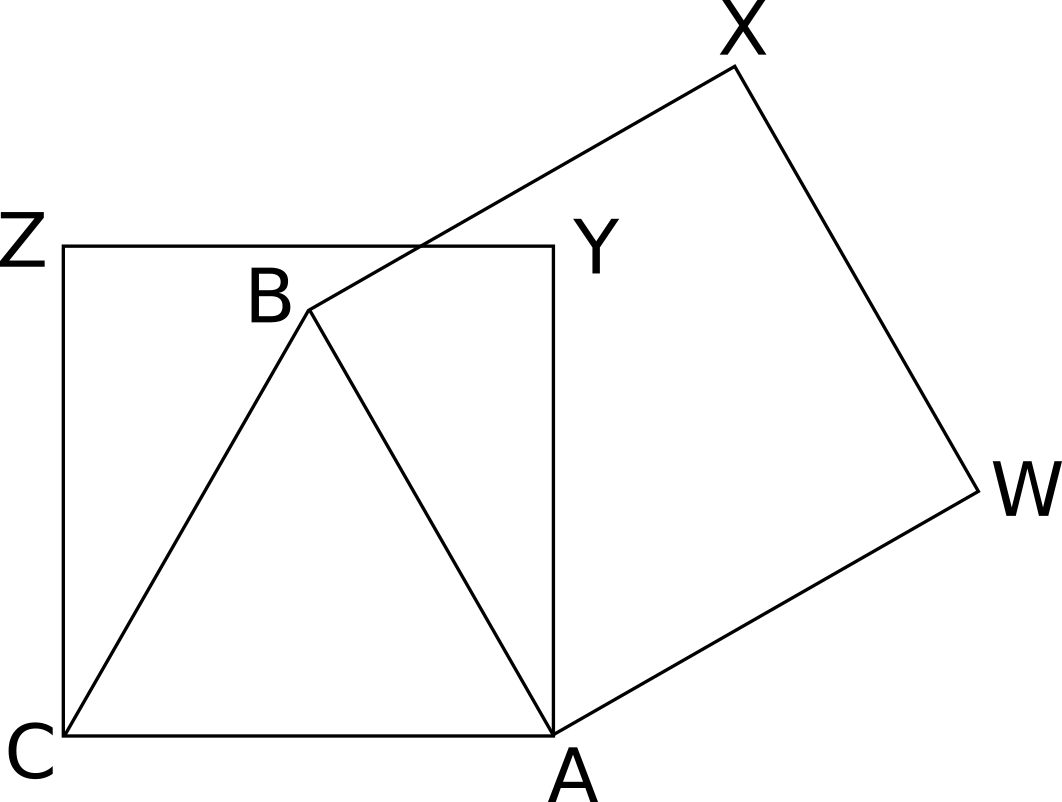
\includegraphics{geometry1_2}
      \caption{Task \ref{squares_task_statement}} \label{squares_task}
    \end{figure}
    \begin{figure}[ht]      
      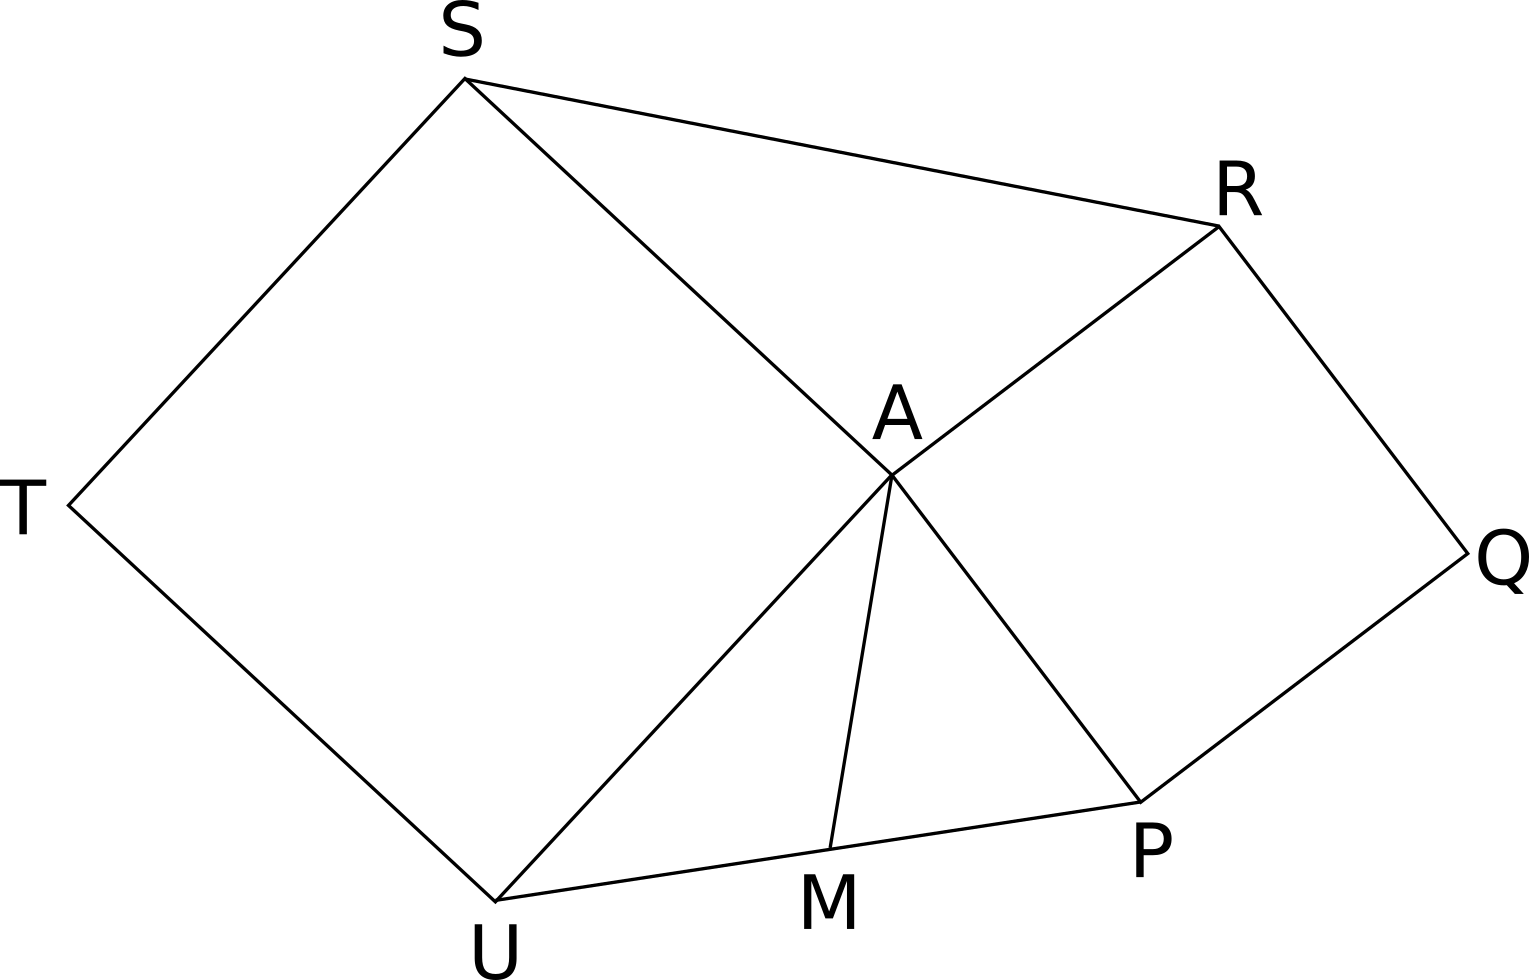
\includegraphics{geometry1_3}
      \caption{Task \ref{wobbly_squares_task_statement}} \label{wobbly_squares_task}
    \end{figure}
  \end{enumerate}
\end{document}
